%!TeX TXS-program:bibliography = txs:///biber
%!TeX program = xelatex
\documentclass[research,19]{idcc}
\usepackage[utf8]{inputenc}
\usepackage{csquotes}
\usepackage{graphicx}
\usepackage{listings}
\usepackage{hyperref}
\hypersetup{
	colorlinks,
	linkcolor={black},
	citecolor={black},
	urlcolor={blue}
}
\usepackage{float}
\usepackage{acronym}
\usepackage{setspace}
\usepackage{etoolbox}

%%% Just comment out one or the other of the "togglefalse/toggletrue" pairs

\newtoggle{final}
\newtoggle{blind}
\togglefalse{final}
%\toggletrue{final}
%\toggletrue{blind}
\togglefalse{blind}


\iftoggle{blind}{
\usepackage{draftwatermark}
\SetWatermarkText{blinded \today}
\SetWatermarkLightness{0.9}
\SetWatermarkScale{0.3}
}{}


\iftoggle{final}{}{
	\usepackage{draftwatermark}
	\SetWatermarkText{SUBMITTED - DO NOT DISTRIBUTE}
	\SetWatermarkLightness{0.9}
	\SetWatermarkScale{0.3}
}


% to read the table
\usepackage{csvsimple}
\usepackage{longtable}
\usepackage{booktabs}
% for adding a flex space to the metajelo macro
\usepackage{xspace}
% to adjust floats
\usepackage{placeins}
% for hyphenating the TT font in the table
\usepackage[htt]{hyphenat}
% better tt font
\usepackage[scaled=0.8]{beramono}
\hyphenation{institution-Sustaina-bility super-Organization-Name institutionPolicy-FreeText}


\input{acrodefs.tex}
%\usepackage{natbib}
%\usepackage[sorting=nyt,maxnames=10,backend=biber]{biblatex}
\usepackage[style=apa,natbib,sortcites,backend=biber,date=year]{biblatex}
\AtEveryBibitem{\clearfield{month}}
\AtEveryBibitem{\clearfield{day}}
%\DeclareLanguageMapping{american}{american-apa}
\DeclareLanguageMapping{british}{british-apa}
\addbibresource{references.bib}
\addbibresource{references-zotero.bib}
\addbibresource{aej-rep.bib}


% Table
\usepackage{array}
\newcolumntype{L}[1]{>{\raggedright\let\newline\\\arraybackslash\hspace{0pt}}p{#1}}
\newcolumntype{C}[1]{>{\centering\let\newline\\\arraybackslash\hspace{0pt}}p{#1}}
\newcolumntype{R}[1]{>{\raggedleft\let\newline\\\arraybackslash\hspace{0pt}}p{#1}}

% Different ways to cite URLS
%\newcommand{\urlcite}[2]{\href{#1}{#2}
\newcommand{\urlcite}[2]{#2\footnote{\url{#1}}}
% 

\newcommand{\metajelo}{\texttt{metajelo}\xspace}

%
% Metadata
\iftoggle{blind}{
	\author{AUTHOR}
	\affil{University}
	\correspondence{Email: \email{blinded@ijpc.net}}
}%
{	% full names only when not blinded
\author{Carl Lagoze}
\affil{University of Michigan}
\author{Lars Vilhuber}
\affil{Cornell University}
\correspondence{Lars Vilhuber. Email: \email{lars.vilhuber@cornell.edu}}
}
\title{metajelo: A metadata package for journals to support external linked objects}

%\conference{14th International Digital Curation Conference}
\submitted{December 2018}



\begin{document}
\maketitle

\begin{abstract}
	\input{abstract}
\end{abstract}

\section{Introduction}
\label{sec:intro}
Reproducibility and replicability of scientific findings has been given great scrutiny in recent years \parencite{CamererScience2016,Collaboration2015-ev,Klein2014,FanelliPNAS2018}.%
\footnote{There is considerable heterogeneity in the use of the terms
	``reproducibility'' and ``replicability''. In this paper, we will adopt
	the following definitions: reproducibility is ``the ability of a
	researcher to duplicate the results of a prior study using the same
	materials and procedures as were used by the original investigator,''
	\parencite{Bollen2015} whereas replicability
	differs in that ``new data are collected.'' (ibidem). See also \cite{NationalAcademiesofSciencesEngineeringandMedicine2019} for a similar definition.}
%
Actual published individual reproductions or replications are notably not very common \parencite[in economics, see][]{BellMiller2013b,Duvendack2017}. In part, this is because it often was difficult to find the materials required to conduct reproducibility or replication exercises \parencite{Dewald1986,McCullough2006,McCullough03}.  

Scientific journals, whether run by publishing companies (Springer, Elsevier, etc.) or learned societies (American Economic Association, Midwest Political Science Association, American Statistical Association, Royal Statistical Society, to name just a few in the social and statistical sciences), have been playing an important role in supporting these efforts for many years \parencite{stodden_enhancing_2016}, and continue to explore novel and better ways of doing so. More and more journals are adopting ``data and code availability'' policies,%
\footnote{In the social sciences, the major economics and political science journals published \acp{DCAP} in the mid-2000s \parencite{American_Economic_Association2008-wayback,nicholaseubankThePoliticalMethodologist2014}.}
though some doubt has been cast on their effectiveness \parencite{stodden_toward_2013,StoddenPNAS2018,Hoeffler2017,ChangAm.Econ.Rev.2017}. Some of the lack of replicability identified by recent studies \parencite{Hoeffler2017a,Chang2017,ChangLi2015,CamererEvaluatingreplicabilitylaboratory2016,StoddenPNAS2018}  occurs despite the fact that journals have  policies that encourage it. One issue is the lack of consistent, reliable metadata on the materials provided to journals, and in particular those supplementary materials, such as data and code, provided through third-party locations.

Several journals have been hosting these ``supplementary materials'' on their own journal websites or on affiliated repositories (e.g., Harvard Dataverse, Figshare) in support of reproducibility of the work described in published scientific articles. In these cases, data and code deposits are requested when authors' work has been (conditionally) accepted after peer review, or, less frequently, as part of the original manuscript submission process. By doing so, these journals assume for themselves (or delegate to a single trusted third party) the curation role for these materials, and assume control of how long these materials are to be preserved and their terms of accessibility.

Some of the lack of replicability identified by recent studies \parencite{Hoeffler2017a,Chang2017,ChangLi2015,CamererScience2016,StoddenPNAS2018}  occurs despite the fact that journals have  policies that encourage the provision of replication packages. Evaluating compliance with policies as well as quality and utility of replication packages is arduous, if not impossible, due to a lack of consistent, reliable metadata on the materials provided to journals. In many cases, while a replication package is provided to the journal, the underlying data are not available within the replication package, due to a mix of non-compliance, legal, and ethical constraints on redistribution of the data. 

XXXXXX leading to renewed calls for better reproducibility \parencite{stodden_enhancing_2016}, broad efforts to better define \acp{DCAP} \parencite{CenterforOpenScience2016,HrynaszkiewiczInt.J.Digit.Curation2017}, and increased enforcement of \acp{DCAP} \parencite{JacobyInsideHigherEd2017,10.1257/pandp.108.745,VilhuberAEAPap.Proc.2019}.

Authors are increasingly being encouraged and trained in reproducible methods from the outset of their research projects \citep{WilsonArXiv160900037Cs2016,Christensen2019a}, rather than describing their data and code much later, \textit{i.e.} after submission to journals. This includes carefully documenting provenance of third-party datasets being used, and properly curating generated datasets (surveys, collected data, etc.) in data archives as soon as possible. Such early deposit allows more time for curation, potentially improving the quality of deposits. However, it conflicts with some (but not all) journal workflows, which integrate data deposit into the article submission process. Prior deposits may not be captured by the same metadata as in-workflow deposits.

Furthermore, in at least some social sciences, the use of pre-existing but non-public data has increased substantially \parencite{Chetty2012} and remains high: \cite{Kingi2018} show about 40\% of economics articles using restricted-access data.  Confidentiality and licensing constraints prevent authors from depositing such data in open archives. Data citation \parencite{DataCitationSynthesisGroup2014} of such data is often challenging. Journals must rely on an increasingly diverse cadre of data-holding institutions, not all of which are or perceive themselves as archives in the traditional sense, while satisfying increasing scrutiny of the provenance of the research results published by them. 

Both scenarios - early and third-party deposit of data and use of restricted-access data - make it difficult for authors and journals to document the full provenance of the data underlying the scientific results in published articles. The resulting lack of transparency in data provenance is detrimental to the overall effort of increasing transparency in the sciences, in particular FAIRness of data access \citep{HagstromFORCE112014}.\footnote{We note that restricted access to data is not inherently incompatible with FAIR, as long as there exists metadata that is FAIR.}

The approach outlined in this article proposes a metadata package, derived from existing metadata schemata where possible, that provides a lightweight approach to ameliorating this problem. In particular, the proposed metadata package, called \metajelo (\underline{meta}data package for \underline{j}ournals to support \underline{e}xternal \underline{l}inked \underline{o}bjects) documents some of the key characteristics that journals care about in the case of supplementary materials that are held by third parties, within the context of FAIR: existence, accessibility, and permanence. Our intent in defining the metadata package is three-fold. First, the package enables  authors to provide the information as they submit articles to journals, allowing informed editorial decisions to be made. Second, at the time of publication, the information is made public, providing robust documentation on data provenance in an immutable package, in a compact fashion.  The package allows for better documentation of any data, regardless of the difficulty of access.   Thus the information provided for less accessible (non-public data) is improved by treating it symmetrically with open access data. Finally, by providing the information in a machine-readable format, the evaluation of compliance with \acp{DCAP} can be more easily assessed systematically. Overall, \metajelo aims to   increase the transparency of what up until now has been very opaque.

We start by providing some background. We describe the use case motivating our approach, with detailed use cases provided in the appendix. We relate our approach to existing metadata, both in terms of structure and of content, and then describe the metadata package. We conclude by discussing some usability issues for three contributors or consumers of this information, and an outlook on a possible implementation.


\section{Background}
\label{sec:background}
In most applied sciences,
it has become common publication practice to provide evidence of the
statistical or laboratory data underlying the conclusions. This is done
to support reproducibility and replicability of the scientific
findings. 
Journals with a
data deposit policy have stored the supplementary materials on journal
websites, often as simple web-based ZIP archives. While ensuring that
the materials are preserved as long as the journal is active
(\textit{permanence}) and are accessible to any reader of the original article (\textit{accessibility}), certain shortcomings became
apparent. Very large datasets and datasets with confidentiality concerns
were nearly always out of scope. 

More recently, journals have leveraged
either dedicated, journal-branded views onto larger archives (e.g,
Dataverse, Figshare), built their own data archive infrastructure
(\urlcite{https://www.elsevier.com/authors/author-services/research-data}{Elsevier/Mendeley}), or have allowed for data and code to be stored
more generally on any of a curated list of trusted%
\footnote{CoreTrustSeal, \url{https://www.coretrustseal.org/}}
or approved
whitelist of third-party repositories.%
\footnote{\url{https://f1000research.com/for-authors/data-guidelines}, \url{https://www.nature.com/sdata/policies/repositories}}
Each of these alternatives rely
on a journal or publisher vetting the repositories and ascertaining
that it meets some set of criteria, or relying on third-party vetting of
repositories exists, such as CoreTrustSeal.%
\footnote{\url{https://www.coretrustseal.org/}} 
For instance, \cite{NatureScientificData2019} assesses relevance to the community, cost to researchers, data access conditions, repository longevity, data persistence and versioning. \cite{CoreTrustSealCoreTrustSeal2017} assesses similar criteria, as well as policies surrounding a set of requirements. The presence on a list of recommended data repositories, or a successful CoreTrustSeal certification, are strong indicators of robust and persistent archives.

However, in our experience \parencite{VilhuberAEAPap.Proc.2020,Kingi2018}, only a few of the holders of restricted-access data appear on such lists. Large survey institutions, many national statistical offices, and nearly all private-sector holders of restricted-access data provide some information about accessibility, but nearly no (publicly accessible) information about data persistence, versioning, or citability of their data assets. While publishers and (some) funders expect that repositories support researchers in making data FAIR, many data providers have yet to respond. In some cases, data access by researchers is incidental, and data providers are not responsive to FAIR considerations, in particular for private sector and sub-national providers of administrative data. Even at the national level,   regulations in various countries that aim to improve access to and preservation of data assets for research are very recent (Digital Economy Act of 2017 in the UK, Loi pour une République Numérique 2017 in France, and the Foundations for Evidence-Based Policymaking Act of 2018 in the United States, to mention only a few examples), and have yet to make a measurable impact. 

Even when data are public-use, or even when the repository is indexed in re3data,\footnote{\url{https://www.re3data.org}} information about accessibility and permanence are incomplete or wrong. Institutions are also able to list multiple access and preservation policies, leaving it open which policy applies to a particular data object. See the Appendix for additional details.

%In all cases known to us, the support for restricted-access
%repositories is quite limited. Thus, most of the known support for
%third-party repositories does not provide much information about
%accessibility (the presumption is that access is open), nor about the
%permanence of the repositories - this is presumably one of the
%evaluation criteria that journals and publishers use, but is not clearly
%defined as such. 
%In fact, at least one of the consulted publishers
%explicitly allows for quite transitory repositories for code, without
%clearly distinguishing that from archives that are more permanent.%
%\footnote{F1000Research (\url{https://f1000research.com/for-authors/data-guidelines}) allows for code deposits through github.com, which has no mandate to preserve, and allows code owners to delete materials at any time without restrictions.}

To a large extent, the onus on reporting on these facets of data archives falls onto the researcher who uses these data, and will continue to do so for considerable time. 
%
Nevertheless, much of the information about persistence of archives and
materials stored within those archives is available, albeit in
idiosyncratic and non-machine readable form. Consider only the case of
national archives (e.g., the \urlcite{https://www.archives.gov/dc/researcher-info}{U.S. National Archives} or the \urlcite{http://www.archives-nationales.culture.gouv.fr/}{\textit{Archives Nationales} in France}). 
In general, data stored in national archives is
permanently archived; if it is not, this is clearly documented.%
\footnote{For instance, the program code for the Business Register is destroyed when a new system is put in place - they are never kept \parencite{U.S.CensusBureau2009}. Unedited master files for the American Community Survey are destroyed 6 years after the Edited master files are verified, unless still needed ``for Census operations'' \parencite{U.S.CensusBureau1999}.}
Furthermore, access is generally not restricted - if it is, this is
clearly documented. However, materials in national archives do have
certain restrictions - they may require sending in a written request, or
a physical visit to a location with copies of the data. Thus, while the
information may satisfy the publication requirements of even the most
open journal, there is no robust and standardized way of documenting the
additional restrictions on access that persist. 

In proposing the
metadata package outlined in this article, we attempt to improve on this
situation. By providing a sparse but sufficient encapsulation of the
information collected from authors, archives, and other third-parties,
we create greater transparency about the data supporting the research.
By relying on existing metadata schemas and metadata content, we
minimize the effort by all parties involved, increasing the likelihood
of adoption. And by intrinsically addressing the possibility that the
information obtained at the time of publication may differ from that returned by later
requests for the same information, we provide the tools to journals,
publishers, and their editors to document that the decision to publish
was based on adequate information at the time of the publication (or
acceptance decision).



\section{Use Case}
\label{sec:usecase}
We target a specific but very common use case (Figure~\ref{fig:usecase}). A researcher has written a paper with empirical content, and is required by the journal's data and code availability policy to prepare a ``replication package.'' The journal's policy requires that the code and data be accessible to others, but does not require deposit of the materials as a ``supplementary file,'' i.e., as a ZIP file on their website.\footnote{In fact, some journals may not offer that option.} However, in all cases, the journal wishes to ascertain three key attributes of the replication package or packages:
\begin{itemize}
    \item the \textit{existence} of the package
    \item the \textit{access rules} to the package (license, terms of use)
    \item the \textit{persistence} of the package
\end{itemize}
In an ideal scenario, the existence of the package can be easily ascertained in a reputable repository, it is made available under an well-specified (ideally open) license, and it is available ``forever''. When the journal manages its own repository, these attributes are known. When the package is available elsewhere, these attributes need to be discovered. Furthermore,  this needs to happen in a scalable,  automated, and reusable fashion, as it should be feasible to do so for all articles, submitted to any journal. However, in our use cases, the data used by the author is in fact re-used, secondary-use data, where the source data may not be in a traditional trusted repository. This, after all, is the whole point of FAIR: to be able to re-use existing data. And yet, the availability of metadata in such cases is problematic. 

\begin{figure}
    \centering
    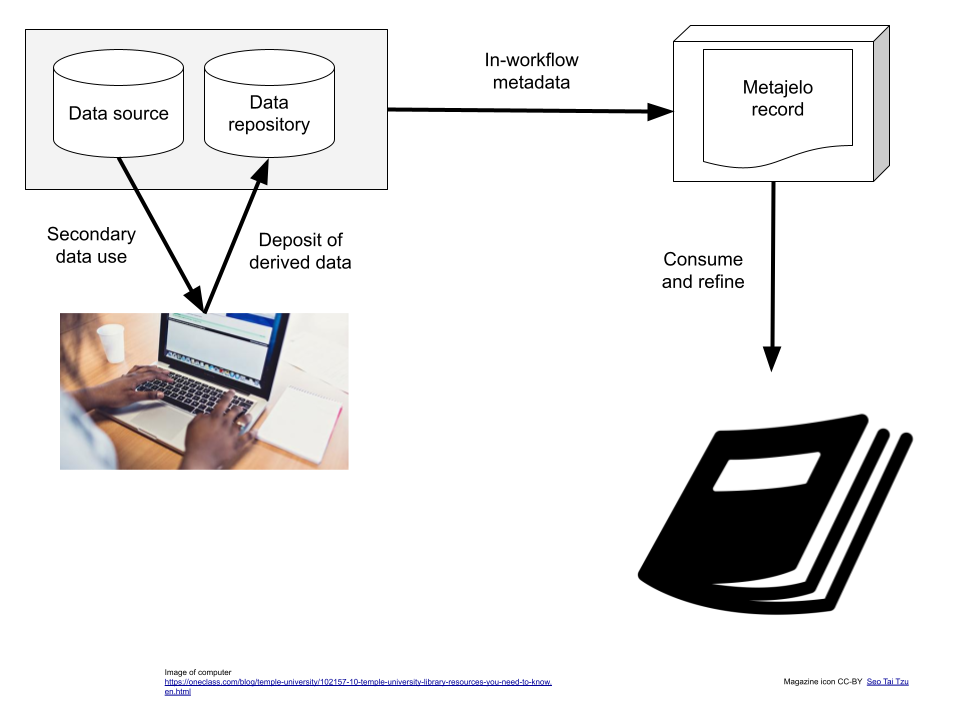
\includegraphics[width=\textwidth]{text/images/metajelo drawing.png}
    \caption{Typical secondary-use of research data}
    \label{fig:usecase}
\end{figure}

\subsection{Current Metadata Infrastructure and Use Cases}
The current metadata infrastructure should be expected to work well for open-access data deposits. Deposits are encouraged in known repositories such as \ac{ICPSR}, Zenodo, or the \urlcite{https://osf.io}{Open Science Framework}, which have been vetted according to certain criteria by the journals themselves.

But what if an author has deposited the information in a reputable but unlisted repository, for instance the \urlcite{https://ada.edu.au/}{Australian Data Archive}? Emails are to be exchanged, and some case-by-case vetting of repositories, their reliability, and whether they assign \ac{DOI} is performed. FAIRsharing.org and re3data are invoked to ascertain their policies. 

In the Appendix, we demonstrate for three cases that this infrastructure - DataCite, re3data, and FAIRsharing - will fail on even simple scenarios. In all cases, we attempt to ascertain \textit{existence}, \textit{access rules} (terms of use and licenses), and \textit{persistence} (preservation policies) via machine-readable metadata. We fail to collect complete information in  all cases. Furthermore, as of the writing of this article, and presumably for some time yet, this infrastructure simply cannot support scenarios that use broadly available restricted-access data. By ``broadly available restricted-access'', we mean that a non-trivial fraction of a research community can be granted access to these data, which are restricted-access only for reasons of confidentiality. This scenario is quite common - it applies to clinical data in psychology as much as demographic data collected by national statistical agencies in every country in the world. 

The three cases are as follows. First, we show that a user-initiated data deposit of a digital  object at  \urlcite{https://www.openicpsr.org}{openICPSR}, properly recorded in DataCite, can at best reveal \textit{existence}, but cannot reveal the remaining attributes (\textit{access rules} and \textit{persistence}) through queries to the infrastructure. A customized parser can ascertain the \textit{license} by querying the landing page of the object. Queries to DataCite fail to elicit the  license because it is optional. Queries to re3data fail because a record cannot be found using information available through the \ac{DOI}, in particular, the name of the repository. Cheating somewhat, when we force a query to re3data's entry for \ac{ICPSR} \parencite{Re3data-icpsr}, it fails to yield correct information, presumably because the record is not maintained by ICPSR staff, and does not hold information on openICPSR policies. We fail to ascertain the preservation policy through queries to all sources, and only subject-matter expertise can find the information on ICPSR's website. 

The second query is for the \ac{PSID} Geospatial Data \parencite{psid-geodata}. The \ac{PSID} is a longitudinal household survey conducted by the University of Michigan, which began in 1968. More than 4000 peer-reviewed publications have used the data \parencite{psid-homepage}. The data are available without cost to researchers - but they do require that terms of use be agreed to before downloading, through registration. This is accurately reflected in the r3data entry for the \ac{PSID} \parencite{Re3data-psid}. However, we are considering the Geospatial Data, which is restricted data. re3data fails to record any information for this access mechanism. Furthermore, although \ac{PSID} has acted as a data curator for its own data for 50 years, it does not assign a \ac{PID} to the data. DataCite has no information on any  \ac{PSID} data holdings, which are only available through the \ac{PSID} website. Until recently, both non-restricted and restricted data could not be deposited at journal websites or other repositories, as per the terms of use.\footnote{This has changed recently with the introduction of an openICPSR-hosted \ac{PSID} repository, but see the issues above.} Finally, although the \ac{PSID} has, of course, a 50-year track record, no statement can be found on the website attesting for preservation plans, or for versioning of data (preservation of prior versions).\footnote{Personal communication in November 2018 with David S. Johnson, at the time Director of the \ac{PSID}, indicates that all versions of non-restricted and restricted data are preserved in a dark archive.}

The third example is a confidential dataset made available by a \ac{NSO}, in this case the U.S. Census Bureau, although it is typical of microdata holdings by \ac{NSO} around the world. The \ac{LBD} \parencite{LBD,MirandaJarmin2002} is one of the most widely used microdata files in the \ac{FSRDC} system. The \ac{FSRDC} system is used by nearly 700 researchers at 29 locations around the United States \parencite{u.s._census_bureau_center_2018}. As with the \ac{PSID}, entries for the U.S. Census Bureau exist on re3data \parencite{Re3data-uscb}, but have no information on the \ac{FSRDC}. No \ac{PID} have yet been assigned to any datasets. Furthermore, no data can be removed from the \ac{FSRDC}. Researchers must thus rely on the U.S. Census Bureau for preservation. In addition to the \ac{LBD} itself, which is presumably covered by a record schedule, detailing its preservation period, researchers also need to consider the preservation of any derivative files they wish to make available as part of their research. If these are aggregated results (model coefficients, etc.), they are released by the U.S. Census Bureau to the researcher. Microdata cannot be released. Most of this information is provided to researchers when they obtain access, but cannot easily be communicated to journal editors or readers of articles. Nevertheless, as we have argued  
\iftoggle{blind}{[BLINDED]}{\parencite{Lagoze2017-qv}} and experienced in our own research 
\iftoggle{blind}{[BLINDED]}{\parencite{AbowdVilhuber2005,AbowdEtAl2009c,McKinneyEtAl:submitted:2017}}, it is definitely feasible to do reproducible research in this environment. The difficulty consists in communicating that information, in a reliable fashion, to editors, referees, and readers.




\subsection{Common Denominator}
We have chosen three types of datasets -- public-use, restricted-access with light restrictions, restricted-access with strong restrictions --, curated by three different institutions -- an open repository, a panel survey  provided by a recognized leader in the field, and confidential business microdata provided by one of the largest and oldest \ac{NSO} in the world -- all with impeccable data curation reputations. The choice is idiosyncratic, but it presumably is symptomatic of the still young state of the metadata infrastructure. We don't believe these examples are exceptions - similar institutions exist all over the world, and we could as easily have done such examples with data from Australia \parencite{PTKLYP_2018}, Germany (Research Data Centre (FDZ) of the German Federal Employment Agency (BA) at the Institute for Employment Research (IAB)). Presumably, counterexamples can be given. But journal editors and authors need such mechanisms to be broadly feasible if they are to use them. At present, that is not the case.

We set out to accomplish this by designing a  metadata package, drawing on existing schema used within the infrastructure, but populating it in a decentralized fashion, at the point of first use: the journal submission system, or if the researcher uses a reproducible workflow, at data acquisition by the researcher. An associated application can leverage the metadata infrastructure where it does provide information,  and pre-fill any fields. However, when ambiguous responses are obtained, or no information is available, the researcher can provide guided or verbatim answers. At both points in time, the researcher has the best incentives to provide the information accurately -- the acceptance of the submission may depend on the accuracy of the information -- and the most timely recollection of where to obtain the information.



\section{Related Metadata and Efforts}
\label{sec:related-metadata}


A number of  initiatives address the issue of reusability of research objects and replicability of science, some of them through proposed metadata standards. None of these efforts can completely provide the information and benefits that our proposed  \metajelo package (described in more detail below) provides. Nevertheless, we have endeavoured to leverage these efforts when possible (i.e., when semantics of tags overlap with our goals and when their XML schema can be cloned for interoperability).%
\footnote{We originally attempted to re-use other schemata by reference, import, and use of name spaces. However, we encountered multiple problems. Name spaces were not handled consistently across parsers. The schemas we intended to re-use were not designed for that purpose. We thus reverted to "re-use by cloning", for lack of robust alternatives.} 
Our hope is that this makes both interoperability with those efforts as easy and possible, and that the use of already established and perhaps familiar tags, attributes, and controlled vocabularies decreases the learning curve for use of our proposed schema.  In the remainder of this section we describe related initiatives and the influence they have on our metadata design.

\subsection{DataCite}
The most related metadata vocabulary comes from \urlcite{https://www.datacite.org/}{DataCite}, which provides infrastructure to locate, identify, and cite research data. Identification is done via the DOI infrastructure for persistent identification, which has emerged as the standard for naming scholarly objects.  The DataCite metadata schema \parencite{DataCiteMetadataWorkingGroup2017a,DataCiteMetadataWorkingGroup2017} specifies elements and attributes to describe data resources for the purpose of citation, location and retrieval.  Because of the notable overlap in the purpose of DataCite  and our proposal, we make use of multiple parts of this schema. Note, however, that DataCite is targeted as describing the data products themselves, where our concern is to register the placement of those products in a repository and ancillary information about that placement. While the DataCite schema has a \texttt{license} field, it is optional, and  often empty. There is no information on more complex access policies, and no information on preservation.

\subsection{Re3data}
The Re3data initiative \parencite{Rucknagel2015,Re3data.Org2015} addresses the goal of describing repositories via an online registry of research data repositories based on a common metadata standard describing such repositories.
%The goal of describing repositories and archives for data curation is directly addressed by the Re3data initiative \parencite{RucknagelMetadataSchemaDescription2015,Re3data.Orgre3dataorgMetadata2015}.  The goal of Re3Data is to support an online registry of research data repositories.   The mechanics underlying this is to establish a common metadata standard for describing such repositories, 
This metadata is then used to power a search interface.  The registry and search interface are targeted at researchers searching for the appropriate repository in which to store their data.
A primary technical output of the work of re3data is a ``Metadata Schema for Description of Research Data Repositories'' now in its 3rd version and expressed as an XML schema.  The schema addresses repository characteristics such as identification,   language, administrative contacts, subject focus, funding basis and the like.  Our work addresses repository characteristics and reuses semantics from the Re3data schema where appropriate and possible.  We will describe the details of this reuse later in this paper.

\subsection{CrossRef}
\urlcite{https://www.crossref.org/}{CrossRef}  sits functionally between our work and the two initiatives described above.  It was conceived by publishers as a DOI registry that, in addition to providing the resolution of those DOIs, stores metadata for the corresponding scholarly object.  An important aspect of this metadata are cross-references (citations) among the named objects \parencite{CrossRef}.  In that sense, CrossRef acts as a ``switchboard'', documenting linkages between scholarly objects. Originally, the linkages were citations between journals, but with increasing interest in data these linkages have been expanded to include these supplementary materials.  In this context, CrossRef collaborates and interoperates with DataCite, with the former focusing on registration and description of journal articles and conference papers, and the latter on data and other supplementary artifacts .  The CrossRef schema is a relatively complex tag set for describing articles.  
%As our intention is to promote a lightweight approach (not necessarily exclusive but perhaps in tandem with CrossRef), we have not directly borrowed from their schema.  Also, our focus is linking to repositories or archives that contain supplementary material, as opposed to the object itself.

\subsection{Scholix}
The Scholix effort \parencite{Burton2017} is also closely related to our proposed package. However, while it may lay the groundwork for the information here, it fundamentally does not have rich enough information about the linked objects to fulfill our core purpose.

\subsection{CoreTrustSeal}
Two additional related initiatives are worthy of mention.   The Core Trustworthy Data Repository Requirements \citep{CoreTrustSealCoreTrustSeal2017} are the result of work within the Research Data Alliance to establish standards for so-called ``trustworthy'' repositories.  These are repositories that meet a set of criteria that deem them dependable for the long-term curation of data.  The criteria are a mixture of technical, administrative, financial, and personnel characteristics.  The criteria are not as of yet, or planned to be, encoded in a machine-readable schema.  Instead, repositories apply for trusted status through a form that his reviewed by a human board of review.  Our proposed metadata format allows for the attribution of a repository as ``trusted'' and thus integrates minimally with the CoreTrustSeal effort. However, as the CoreTrustSeal does not provide an \ac{API}, the information embedded within the certification cannot be re-used. Furthermore, as noted for re3data, an institution may have multiple policies, and it may not always be easy to attribute a particular policy to a particular object.  

\subsection{JATS}
The \urlcite{https://jats.nlm.nih.gov/}{JATS (Journal Article Tag Suite)}, led by the NCBI (National Center for Biotechnology Information) aims to develop specifications for standardized (XML) markup for scholarly articles.  The effort grows out of work done on so-called ``NLM DTDS'', which modelled tag sets for scholarly document structuring.  \urlcite{https://jats4r.org/}{JATS4R} (JATS for reuse) is a follow-on effort, designed to reuse and extend XML models defined by JATS, with the primary goal of facilitating reuse of existing scholarly material (publications and supplementary data). The result is a set of models specifying document structure, rather than simply metadata.  The structural elements address issues such as how to mark-up authors and affiliations, citations, data citations and the like.

\subsection{Data Accessibility Statements}
The Belmont Forum published a template ``Data Availability Policy and Statement'' \citep{murphy_fiona_2018_1476871}, with similar goals as our project, though the focus seems to be primarily on human-readable statements.


\section{Metadata Package}
\label{sec:metadata-package}
\label{sec:approach}
The high-level structure of our proposed metadata package is illustrated in the Figure~\ref{fig:schema_v1} (produced by OxygenXML). 
\begin{figure}
	\includegraphics[width=\textwidth]{images/Selection_447.png}
	\includegraphics[width=\textwidth]{images/Selection_448.png}
	\caption{\label{fig:schema_v1}High-level structure of proposed package}
\end{figure} 
As shown, each package is structured as a record, which conceptually models a linkage between a publication and its supplementary materials.  As shown, a record has an identity (\ac{DOI}), a date created, a last modified date, and the identity (\ac{DOI}) of the research objects (papers) that are associated with the supplementary products.
Each record then can describe an unlimited number of \texttt{supplementaryProducts}.  Each product has an identifier, a description of its type, licensing information, and linkages to full metadata available elsewhere that fully describes the product.  Each \texttt{supplementaryProduct} has an associated location block, which contains information about the institutional archive at which the respective \texttt{supplementaryProduct} is located.  Finally, for each institution, the set of possible policies are listed, with a boolean designation of the applicability of a policy to the respective supplementary object.   
The full annotated schema is available for examination online at 
\iftoggle{blind}{[URL blinded - please contact JOURNAL]}{\href{https://github.com/labordynamicsinstitute/metajelo}{github.com/labordynamicsinstitute/metajelo}}.

%%%%%%%%%%%%%%%%%%%%%%%%%%%%%%%%%%%%%%%%%%%%%%%%%%%%%%%%%%%%%%%%%%%%%%
%
%%%%%%
%%%%%%          TABLE Metajelo Description
%%%%%%
%%id;field;description;comment;source;larscomment
%\csvreader[/csv/separator=semicolon,/csv/head=true,%
%/csv/before reading=\footnotesize%
%\setlength{\tabcolsep}{2.5pt},%
%/csv/after reading=\normalsize,%
%/csv/head to column names=true,%
%/csv/longtable=llp{3in}@{\hskip 0.2in}p{1in}p{0.5in},
%/csv/table head=%
%\multicolumn{5}{c}{Table~\thetable : \metajelo Description\label{tab:desc:metajelo}}\\%
%\toprule \bf ID & \bf Field &\bf Definition & \bf Notes  &\bf Source \\\midrule\endfirsthead%
%\multicolumn{5}{c}{Table~\ref{tab:desc:metajelo} : \metajelo Description}\\%
%\toprule \bf ID & \bf Field &\bf Definition & \bf Notes & \bf Source\\\midrule\endhead%
%%\bottomrule
%\endlastfoot%
%\midrule&&&\multicolumn{2}{r}{(cont)}\\\endfoot,
%/csv/late after line=\\\midrule,
%%table foot=\bottomrule%
%]%
%{../schema/tabular-metajelo.csv}{}{%
%	\id &\multicolumn{4}{l}{\texttt{\field}:}\\
%	&\  &\description & \raggedright \comment & \source 
%}

\begin{table}
	\centering
	\caption{\metajelo Description\label{tab:desc:metajelo}  }
	
%\input{text/idcc2019-table1}
	
\end{table}
%%%%%%%%%%%%%%%%%%%%%%%%%%%%%%%%%%%%%%%%%%%%%%%%%%%%%%%%%%%%%%%%%%%%%

We highlight a few key elements. First, much of the information about the object itself mirrors the DataCite schema \parencite{DataCiteMetadataWorkingGroup2017,DataCiteMetadataWorkingGroup2017a}, even if no \ac{DOI} exists. The bibliographic metadata schema is based on DataCite for simplicity, and is always required. Much of the information on the institution, including its policies, mirrors the re3data schema \parencite{Re3data.Org2015,Rucknagel2015}, with much simplification. In particular, we are interested primarily in \texttt{policyType="Preservation Policy"} and \texttt{policyType="Terms of Use"}. In contrast with the re3data schema, we have merged licenses into the same repeatable element, so that \texttt{policyType="License"} is a valid option. In all cases, we also allow for verbatim capture of the text of the policy, since policies posted on websites, and not versioned, may change over time. We envision either manual entry by the researcher, or webscraping of the provided policy {URL} to populate this field.
\FloatBarrier
\section{Usability Notes}
\label{sec:usability}
Academic publishing outsources much of the content-related work to authors and subject matter editors. In order to be useful, the proposed package needs tools around it. We sketch out two such tools, and also address the role archives and repositories themselves play. 
\subsection{Metadata ingest}

We envision that the package be provided as a single file during the manuscript submission process by the author. This ensures that existing editorial workflow packages can seamlessly track the package, without needing upgrades to understand the content. Systems that do know how to ingest the information should do so, but are able to collect the information more efficiently. The package can be inspected by curation specialists and data editors and made available to reviewers as needed, and will follow the main document throughout the review process. 
           
\subsection{Creation by authors}
In order to create the package, we envision a simple website, which helps authors fill in the required information.\footnote{A demonstration project is available at \href{https://labordynamicsinstitute.github.io/metajelo-ui/}{labordynamicsinstitute.github.io/metajelo-ui}, archived as \citet{brandon_elam_barker_2021_4509001}.} Appropriate \ac{HCI} testing would need to be done to determine the optimal structure. However, the starting point is the DOI of the object being described, if available, or a bibliographic record, otherwise. From the DOI, a backend query to DataCite or CrossRef can reveal the hosting institution's institutionID. In turn, lookup in re3data or fairsharing.org will reveal elements of the institutional policies with regards to general access or preservation. Institutions often have multiple access policies and licenses, and which one applies to the object identified by the DOI may be hard to determine automatically. The author will be able to choose the appropriate license she consented to from a set of choices appropriate for the object and its hosting institution. In theory, all such information is provided through re3data, but failing to look up complete or accurate information, the author can also fill in the information manually. 
           
\subsection{Hosting by journals}
Journals are expected to post the package on their website, on the same landing page as the article itself. By doing so, the package itself can be parsed by appropriate tools.\footnote{A demonstration project is available at \href{https://labordynamicsinstitute.github.io/metajelo-web/}{labordynamicsinstitute.github.io/metajelo-web/}, archived as \citet{brandon_elam_barker_2021_4507862}.}  Naturally, more complex journal websites can include the contents in the page source code or in their \ac{CMS}. 

\subsection{Decentralizing the linkage architecture}
A final point is worth highlighting. When journals adopt the \metajelo package,  much information will be made available at a key point in the scientific cycle, when incentives are aligned: at the point of publication. By having authors themselves, possibly with help from the editors, create the linkage information (linking data and code archives to articles), having them describe what they know of access and retention policies at archives, creates information on thousands of articles every year, across hundreds of journals. This information can be harvested. Clearly, not all of the information will be accurate or consistent - but neither is the information currently being curated in centralized repositories of such information. Disambiguation algorithms will need to be deployed, and aggregation needs to allow for multiple (non-authoritative) answers. Facilities like Re3data will become aggregators instead of creators of such metadata. Our hypothesis is that the error rate in metadata will decline, but not disappear. 

\section{Acknowledgements}
\label{sec:ack}
\iftoggle{blind}{[Acknowledgements blinded.]}{
Lagoze and Vilhuber acknowledge funding received from \href{http://www.nsf.gov/awardsearch/showAward.do?AwardNumber=1131848}{NSF Grant \#1131848} (NCRN) and the American Economic Association, as well as the Alfred P. Sloan foundation. The views and recommendations expressed herein are those of the authors, and not those of either the American Economic Association or the National Science Foundation.}


%\bibliographystyle{chicagoa}
%\bibliography{references.bib}
\printbibliography


%\appendix
\FloatBarrier
\section{Appendix: Detailed Use Cases}
\label{app:cases}

\newcommand{\suppDir}{supplementary_materials}
\input{\suppDir/usecase-appendix}
\FloatBarrier
%\section{Appendix: Full query response for Use Case 1}
%\lstinputlisting[language=xml]{\suppDir/datacite-api-100590.xml}
\end{document}